%% Topology of ternary complex dimer
%% FigS4TopologyTCDimerSupp.tex
%% Unused packages and definitions removed; TikZ/PGFPlots source formatted.

\documentclass{standalone}

\usepackage{latexsym}
\usepackage{tikz}

\def \half {\frac{1}{2}}

\begin{document}

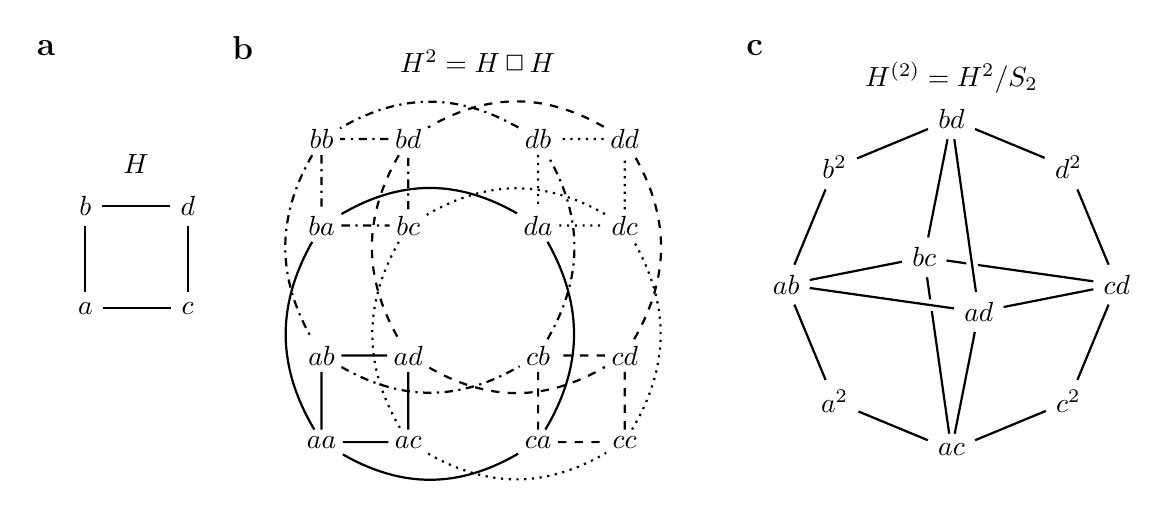
\begin{tikzpicture}[scale=1,style=thick,shorten >=0pt,shorten <=0pt]

    \begin{scope}[xshift=-3cm,yshift=3cm,node distance=1.3cm]
        \node (LRA) {$b$};
        \node[below of=LRA] (RA) {$a$};
        \draw[thick] (LRA) to node[left] {} (RA);
        \node[right of=RA] (RAG) {$c$};
        \draw[thick] (RA) to node[below] {} (RAG);
        \node[right of=LRA] (LRAG) {$d$};
        \draw[thick] (LRAG) to node[] {} (LRA);
        \draw[thick] (RAG) to node[right] {} (LRAG);
        \path (LRA) to node[above,yshift=8pt] {$H$} (LRAG);
    \end{scope}

    \def\r{1}
    \begin{scope}[scale=1.1,xshift=0cm,yshift=0cm,inner sep=2pt]
        \coordinate (titleA) at (1.8,4.4);
        \draw (titleA) node {$H^{2}= H\,\Box\, H$};
        \begin{scope}[xshift=0cm,yshift=0cm]
            \draw (0,0) node[] (aa) {$aa$};
            \draw (\r,\r) node[] (ad) {$ad$};
            \draw (\r,0) node[] (ac) {$ac$};
            \draw (0,\r) node[] (ab) {$ab$};
            \draw[thick] (aa) to (ac) to (ad) to (ab) to (aa);
        \end{scope}
        \begin{scope}[xshift=2.5cm,yshift=2.5cm]
            \draw (0,0) node[] (da) {$da$};
            \draw (\r,\r )node[] (dd) {$dd$};
            \draw (\r,0) node[] (dc) {$dc$};
            \draw (0,\r) node[] (db) {$db$};
            \draw[dotted] (da) to (dc) to (dd) to (db) to (da);
        \end{scope}
        \begin{scope}[xshift=0cm,yshift=2.5cm]
            \draw (0,0) node[] (ba) {$ba$};
            \draw (\r,\r) node[] (bd) {$bd$};
            \draw (\r,0) node[] (bc) {$bc$};
            \draw (0,\r) node[] (bb) {$bb$};
            \draw[dashdotted] (ba) to (bc) to (bd) to (bb) to (ba);
        \end{scope}
        \begin{scope}[xshift=2.5cm,yshift=0cm]
            \draw (0,0) node[] (ca) {$ca$};
            \draw (\r,\r) node[] (cd) {$cd$};
            \draw (\r,0) node[] (cc) {$cc$};
            \draw (0,\r) node[] (cb) {$cb$};
            \draw[dashed] (ca) to (cc) to (cd) to (cb) to (ca);
        \end{scope}
        \draw[thick,outer sep=0pt,inner sep=0pt] (aa) to[bend right=30] (ca);
        \draw[thick,outer sep=0pt,inner sep=0pt] (ca) to[bend right=30] (da);
        \draw[thick,outer sep=0pt,inner sep=0pt] (da) to[bend right=30] (ba);
        \draw[thick,outer sep=0pt,inner sep=0pt] (ba) to[bend right=30] (aa);
        \draw[dashdotted,outer sep=0pt,inner sep=0pt] (ab) to[bend right=30] (cb);
        \draw[dashdotted,outer sep=0pt,inner sep=0pt] (cb) to[bend right=30] (db);
        \draw[dashdotted,outer sep=0pt,inner sep=0pt] (db) to[bend right=30] (bb);
        \draw[dashdotted,outer sep=0pt,inner sep=0pt] (bb) to[bend right=30] (ab);
        \draw[dashed,thick,outer sep=0pt,inner sep=0pt] (ad) to[bend right=30] (cd);
        \draw[dashed,thick,outer sep=0pt,inner sep=0pt] (cd) to[bend right=30] (dd);
        \draw[dashed,thick,outer sep=0pt,inner sep=0pt] (dd) to[bend right=30] (bd);
        \draw[dashed,thick,outer sep=0pt,inner sep=0pt] (bd) to[bend right=30] (ad);
        \draw[dotted,thick,outer sep=0pt,inner sep=0pt] (ac) to[bend right=30] (cc);
        \draw[dotted,thick,outer sep=0pt,inner sep=0pt] (cc) to[bend right=30] (dc);
        \draw[dotted,thick,outer sep=0pt,inner sep=0pt] (dc) to[bend right=30] (bc);
        \draw[dotted,thick,outer sep=0pt,inner sep=0pt] (bc) to[bend right=30] (ac);
    \end{scope}

    \begin{scope}[xshift=8cm,yshift=2cm,scale=0.7,shorten >=0pt,shorten <=0pt]
        \coordinate (title) at (90:3.75);
        \draw (title) node {$H^{(2)}=H^2/S_2$};
        %\draw (title) node {$H^{(2)}$:};
        \draw (0:3) node[] (cd) {$cd$};
        \draw (45:3) node[] (d2) {$d^2$};
        \draw (90:3) node[] (bd) {$bd$};
        \draw (135:3) node[] (b2) {$b^2$};
        \draw (180:3) node[] (ab) {$ab$};
        \draw (225:3) node[] (a2) {$a^2$};
        \draw (270:3) node[] (ac) {$ac$};
        \draw (315:3) node[] (c2) {$c^2$};
        \draw (315:0.7) node[] (ad) {$ad$};
        \draw (135:0.7) node[] (bc) {$bc$};
        \draw[thick] (a2) -- (ab);
        \draw[thick] (ab) -- (b2);
        \draw[thick] (b2) -- (bd);
        \draw[thick] (bd) -- (d2);
        \draw[thick] (d2) -- (cd);
        \draw[thick] (cd) -- (c2);
        \draw[thick] (c2) -- (ac);
        \draw[thick] (ac) -- (a2);
        \draw[thick] (bc) -- (bd);

        \draw[thick] (ad) -- (ac);
        \draw[thick] (ac) -- (bc);
        \draw[thick] (ab) -- (bc);
        \draw[thick] (bc)-- (cd);
        \draw[thick] (cd) -- (ad);
        \draw[thick] (ad)-- (ab);
        \draw[line width=4pt,white] (bd) -- (ad);  \draw[thick] (bd) -- (ad);
        \draw[line width=4pt,,white] (ad)-- (ab);  \draw[thick] (ad)-- (ab);
    \end{scope}

    \def\height{5}
    \def\left{-3.5}
    \draw (\left,\height) node[font=\large] {{\bf a}};
    \draw (\left+2.5,\height) node[font=\large] {{\bf b}};
    \draw (\left+9,\height) node[font=\large] {{\bf c}};

\end{tikzpicture}

\end{document}

